% !TeX spellcheck = fr_CH

% TODO: Replace scan images with clean text where possible

\documentclass[a4paper, 10pt]{report}

\usepackage[french]{babel}
\usepackage[T1]{fontenc}

\usepackage{amsmath, amssymb, amsfonts}

\usepackage{hyperref}
\usepackage{geometry}

\usepackage{xcolor}
\usepackage{graphicx}

\usepackage{fancyhdr}
\usepackage{lastpage}

\usepackage{enumitem}

\geometry{
	a4paper,
	left=25mm,
	right=25mm,
	top=35mm,
	bottom=25mm,
	headsep=5mm,
	headheight=20mm,
}

\definecolor{solution}{HTML}{E5E4E2}
\providecommand{\abs}[1]{\lvert#1\rvert}
\providecommand{\norm}[1]{\lVert#1\rVert}

\begin{document}
		
	\renewcommand{\headrule}{
	\color{lightgray} \par\noindent\rule{\textwidth}{2pt}
	}	
	\pagestyle{fancy}
	\fancyhf{}
	
	\fancyhead[L]{\small \slshape Automne 2024}
	\fancyhead[C]{\Large \bfseries Algèbre I - Série 01}
	\fancyhead[R]{\small Buff Mathias}
	\fancyfoot[L]{
		\small Source files available at:
		\href{https://github.com/MathiasBuff/bsc-math}
		{github.com/MathiasBuff/bsc-math}
		}
	\fancyfoot[R]{
		\small Page \thepage
		\hspace{1pt} /
		\pageref*{LastPage}
		}
	
	\noindent
	\textbf{Exercice 1.} (Résolution graphique de systèmes)
	
	\begin{enumerate}[label=(\alph*)]
		\item Dans l'espace $\mathbb{R}^2$ muni des
		coordonnées cartésiennes$(x, y)$, dessiner
		les droites d'équations
		%
		\[
			3x + y + 1 = 0, \quad
			3x + y = 0, \quad
			\text{et} \quad
			x + 3y = 0
		\]
	
		\item Dans l'espace $\mathbb{R}^3$ muni des
		coordonnées cartésiennes $(x, y, z)$,
		dessiner les plans d'équations
		%
		\[
		x + y + z = 1 \quad
		\text{et} \quad
		x + 2y = 3
		\]
		%
		ainsi que l'intersection des deux plans d'équations
		%
		\[
		x + 2y + 3z = 6 \quad
		\text{et} \quad
		z = 1
		\]
	\end{enumerate}

	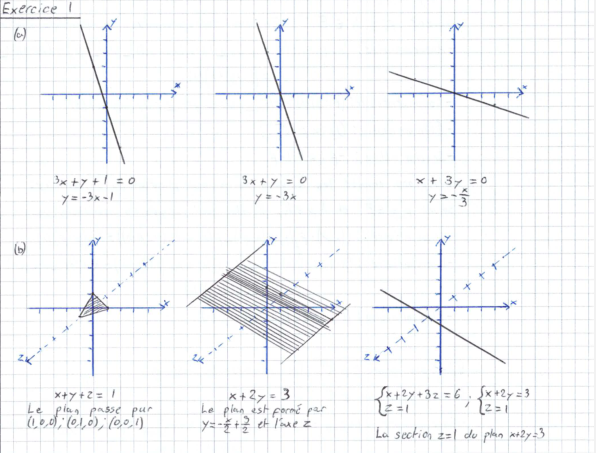
\includegraphics{ex01.png}
	
	\newpage
	
	\fancyhf{}
	\renewcommand{\headrule}
		{\rule{\textwidth}{0pt}}
	\fancyfoot[R]{
		\small Page \thepage
		\hspace{1pt} /
		\pageref*{LastPage}
	}
	
	\noindent
	\textbf{Exercice 2.} (Résolution algébrique de systèmes)
	
	\indent Résoudre les systèmes linéaires suivants
	%
	\[
		\left\{
		\begin{aligned}
			&x + y + z &&= 1\\
			&x &&= \frac{1}{2}
		\end{aligned}
		\right.
		\quad \text{et} \quad
		\left\{
		\begin{aligned}
			&x + y &&= 0\\
			&x - 2y &&= 6\\
			&2x + 3y &&= 0
		\end{aligned}
		\right.
	\]
	
	\colorbox{solution}
	{
		\begin{minipage}{0.9\textwidth}
			\[
				\left\{
				\begin{aligned}
					&x + y + z &&= 1 \quad (-L_2)\\
					&x &&= \frac{1}{2}
				\end{aligned}
				\right.
				\quad
				\left\{
				\begin{aligned}
					&y + z &&= \frac{1}{2}\\
					&x &&= \frac{1}{2}
				\end{aligned}
				\right.
				\qquad
				\left.
				\begin{aligned}
					&x = \tfrac{1}{2}\\
					&y = \tfrac{1}{2} - z\\
					&z = z
				\end{aligned}
				\right.
			\]
			
			\[
				Sol =\{(\tfrac{1}{2}, \tfrac{1}{2} - t, t),
					t \in \mathbb{R}\}
			\]
			
			\vspace{5mm}
			
			\[
			\left\{
			\begin{aligned}
				&x + y &&= 0\\
				&x - 2y &&= 6 \quad (-L_1)\\
				&2x + 3y &&= 0 \quad (-2L_1)
			\end{aligned}
			\right.
			\quad
			\left\{
			\begin{aligned}
				x + y &= 0\\
				- 3y &= 6\\
				y &= 0
			\end{aligned}
			\right.
			\quad
			\left\{
			\begin{aligned}
				x + y &= 0\\
				y &= -2\\
				y &= 0
			\end{aligned}
			\right.
			\]
			
			\begin{center}
				$L_2$ et $L_3$ présentent une contradiction, donc
				$Sol =\emptyset$
			\end{center}
		\end{minipage}
	}
	
	\vspace{5mm}
	\noindent
	\textbf{Exercice 3.} (Espaces vectoriels des fonctions)
	
	\begin{enumerate}[label=\arabic*.]
		\item Soit $E = \mathcal{F}(\mathbb{R}, \mathbb{R})$
		l'ensemble des fonctions de $\mathbb{R}$ vers $\mathbb{R}$.
		Montrer que cet ensemble, muni des lois
		%
		\[
			\begin{aligned}
				&(f + g)(x) := f(x) + g(x),
				\qquad
				& &\forall f, g \in \mathcal{F}(\mathbb{R}, \mathbb{R}),
				x \in \mathbb{R}\\
				&(\lambda \cdot f)(x) := \lambda \cdot f(x),
				\qquad
				& &\forall f \in \mathcal{F}(\mathbb{R}, \mathbb{R}),
				\lambda \in \mathbb{R}, x \in \mathbb{R}
			\end{aligned}
		\]
		%
		où le $+$ et le $\cdot$ du côté droit dénotent l'addition
		et la multiplication usuelles dans $\mathbb{R}$, forme un
		espace vectoriel sur $\mathbb{R}$.
		
		\colorbox{solution}
		{
			\begin{minipage}{0.9\textwidth}
				Vérifions pour $E = \mathcal{F}(\mathbb{R}, \mathbb{R})$
				les axiomes de l'addition :\\
				Soient $f, g, h \in E$
				\begin{itemize}
					\item Associativité : 
						\[
							\begin{aligned}
								(f + (g + h))(x)
								&= f(x) + (g + h)(x)
								= f(x) + g(x) + h(x)
								= (f + g)(x) + h(x)\\
								&= ((f + g) + h)(x)
							\end{aligned}
						\]
					\item Commutativité :
						\[
							(f + g)(x)
							= f(x) + g(x)
							= g(x) + f(x)
							= (g + f)(x)
						\]
					\item L'élément neutre additif $0_E$ est la fonction
					constante $f(x) = 0$.
					\item L'inverse additif est la fonction
					$-f := (-1) \cdot f$
				\end{itemize}
				
				\vspace{5mm}
				Vérifions ensuite les axiomes de la multiplication par
				un scalaire:\\
				Soient $f, g \in E$ et $\lambda, \mu \in \mathbb{R}$
				\begin{itemize}
					\item Associativité : 
					\[
						((\lambda \cdot \mu) \cdot f)(x)
						= (\lambda \cdot \mu) \cdot f(x)
						= \lambda \cdot (\mu \cdot f(x))
						= \lambda \cdot (\mu \cdot f)(x)
					\]
					\item Distributivité :
					\[
					\begin{aligned}
						(\lambda \cdot (f + g)(x)
						&= \lambda \cdot (f + g)(x)
						= \lambda \cdot (f(x) + g(x))
						= \lambda \cdot f(x) + \lambda \cdot g(x)\\
						&= ((\lambda \cdot f) + (\lambda \cdot g))(x)
					\end{aligned}
					\]
					\item Élément neutre : $(1 \cdot f)(x) =
						1 \cdot (f(x)) = f(x)$.
					$-f := (-1) \cdot f$
				\end{itemize}
			\end{minipage}
		}
		
		\item Soit $\mathbb{R}^{\mathbb{N}}$ l'ensemble de toutes
		les suites de scalaires
		$(u_n)_{n \in \mathbb{N}}, u_n \in \mathbb{R}$, qui peut
		aussi être vu comme l'ensemble des fonctions
		$\mathcal{F}(\mathbb{N}, \mathbb{R})$. Montrer que cet
		ensemble, muni des lois
		%
		\[
			\begin{split}
				(u_n)_{n \in \mathbb{N}} + (v_n)_{n \in \mathbb{N}} &:=
				(u_n + v_n)_{n \in \mathbb{N}},\\
				\alpha \cdot (u_n)_{n \in \mathbb{N}} &:=
				(\alpha \cdot u_n)_{n \in \mathbb{N}}
				\qquad
				\forall \alpha \in \mathbb{R},
			\end{split}
		\]
		%
		forme un espace vectoriel sur $\mathbb{R}$.
		
		\colorbox{solution}
		{
			\begin{minipage}{0.9\textwidth}
				Vérifions pour $E = \mathbb{R}^{\mathbb{N}}$
				les axiomes de l'addition :\\
				Soient $u, v, w \in E$
				\begin{itemize}
					\item Associativité : 
					\[
					\begin{aligned}
						(u_n)_{n \in \mathbb{N}} + (v_n + w_n)_{n \in \mathbb{N}}
						&= (u_n + (v_n + w_n))_{n \in \mathbb{N}}
						= (u_n + v_n + w_n)_{n \in \mathbb{N}}\\
						&= ((u_n + v_n) + w_n)_{n \in \mathbb{N}}
						= (u_n + v_n)_{n \in \mathbb{N}} + (w_n)_{n \in \mathbb{N}}
					\end{aligned}
					\]
					\item Commutativité :
					\[
						(u_n)_{n \in \mathbb{N}} + (v_n)_{n \in \mathbb{N}}
						= (u_n + v_n)_{n \in \mathbb{N}}
						= (v_n + u_n)_{n \in \mathbb{N}}
						= (v_n)_{n \in \mathbb{N}} + (u_n)_{n \in \mathbb{N}}
					\]
					\item L'élément neutre additif $0_E$ est la suite
					constante $u_n = 0 \quad \forall n \in \mathbb{N}$.
					\item L'inverse additif est la suite
					$-(u_n)_{n \in \mathbb{N}} := (-1) \cdot (u_n)_{n \in \mathbb{N}}$
				\end{itemize}
				
				\vspace{5mm}
				Vérifions ensuite les axiomes de la multiplication par
				un scalaire:\\
				Soient $u, v \in E$ et $\lambda, \mu \in \mathbb{R}$
				\begin{itemize}
					\item Associativité : 
					\[
					\begin{aligned}
						(\lambda \cdot \mu) \cdot (u_n)_{n \in \mathbb{N}}
						&= ((\lambda \cdot \mu) \cdot u_n)_{n \in \mathbb{N}}
						= (\lambda \cdot \mu \cdot u_n)_{n \in \mathbb{N}}
						= (\lambda \cdot (\mu \cdot u_n))_{n \in \mathbb{N}}\\
						&= \lambda \cdot (\mu \cdot u_n)_{n \in \mathbb{N}}
					\end{aligned}
					\]
					\item Distributivité :
					\[
					\begin{aligned}
						\lambda \cdot (u_n + v_n)_{n \in \mathbb{N}}
						&= (\lambda \cdot (u_n + v_n))_{n \in \mathbb{N}}
						= (\lambda \cdot u_n
							+ \lambda \cdot v_n)_{n \in \mathbb{N}}\\
						&= (\lambda \cdot u_n)_{n \in \mathbb{N}}
							+ (\lambda \cdot v_n)_{n \in \mathbb{N}}
					\end{aligned}
					\]
					\item Élément neutre :
					$1 \cdot (u_n)_{n \in \mathbb{N}}
					= (1 \cdot u_n)_{n \in \mathbb{N}}
					= (u_n)_{n \in \mathbb{N}}$.
				\end{itemize}
			\end{minipage}
		}
		
	\end{enumerate}

	\vspace{5mm}
	\noindent
	\textbf{Exercice 4.} (Notion d'espace vectoriel)
	
	\indent Pour chacun des espaces suivants, dire si c'est un espace
	vectoriel ou non sur $\mathbb{R}$. Si oui, prouver la (les)
	propriété(s) entre parenthèse demandée(s). Si non, expliquer quel
	axiome est mis en défaut. Attention, certaines questions
	n'admettent pas pour réponse juste oui ou non.
	
	\begin{enumerate}[label=\arabic*.]
		\item L'espace $E = \{0\}$ avec les lois usuelles.
			$\rightsquigarrow$ (Neutre de l'addition)
		%
		\item L'espace $E = [0, 1]$ avec les lois usuelles.
			$\rightsquigarrow$ (Neutre de la multiplication)
		%
		\item L'espace $E = \mathbb{Z} = \{..., -1, 0, 1, 2, ...\}$
		avec les lois usuelles.
			$\rightsquigarrow$ (Commutativité de l'addition)
		%
		\item L'espace $E = \mathbb{R}^2$ avec
		l'addition $(x_1, y_1) + (x_2, y_2) = (x_1 + y_1, x_2 + y_2)$ et
		la multiplication $\lambda \cdot (x, y) = (\lambda x, 0)$.
			$\rightsquigarrow$ (Associativité de l'addition)
		%
		\item L'espace $E = \{f : \mathbb{R} \rightarrow \mathbb{R} \mid f(a) = b\}$
		avec les lois usuelles (définies pour l'exercice 3.1),
		où $a \in \mathbb{R}$ et $b \in \mathbb{R}$ sont fixés.
			$\rightsquigarrow$ (toutes les propriétés)
		%
		\item L'espace $E = \mathbb{R}[x]$ des polynômes
		$p : \mathbb{R} \rightarrow \mathbb{R}$ sans borne sur leur degré,
		avec les lois usuelles.
			$\rightsquigarrow$ (Distributivité à droite)
	\end{enumerate}
	
	
	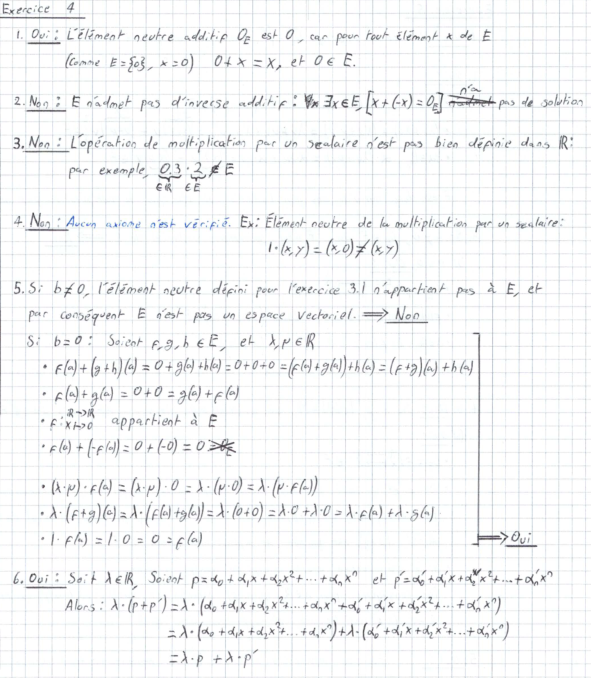
\includegraphics{ex04.png}

	\newpage
	\vspace{5mm}
	\noindent
	\textbf{Exercice 5.} (Notion de sous-espace vectoriel)
	
	\indent Pour chacun des espaces suivants, dire si $F$ est un espace
	vectoriel de $E$ ou non, et le prouver. Tous les espaces vectoriels
	$E$ sont sur $\mathbb{R}$.
	
	\begin{enumerate}[label=\arabic*.]
		\item $E = M_{2, 2}(\mathbb{R}), F = \bigg\{ A \in E
			\mid A = 
			\begin{pmatrix}
				1& a\\
				0& b\\
			\end{pmatrix}
			, \quad a, b \in \mathbb{R} \bigg\}$
		%
		\item $E = \mathbb{R}^3, F = \{\lambda u + \mu v \mid
			\lambda \in \mathbb{R}, \mu \in \mathbb{R}\}$,
		où $u, v \in \mathbb{R}^3$ sont fixés.
		%
		\item $E = \{f : [0, 2\pi] \rightarrow \mathbb{R} \mid
			f(0) = f(2\pi)\}, F = \{f : [0, 2\pi] \rightarrow
			\mathbb{R} \mid f(0) = f(2\pi) = a\}$,
		où $a \in \mathbb{R}$ est fixé.
		%
		\item $E = \mathcal{F}(\mathbb{R}, \mathbb{R})$, et
			\begin{enumerate}[label=(\alph*)]
				\item $F_1 = \{f : \mathbb{R} \rightarrow \mathbb{R}
					\mid \forall x \in \mathbb{R}, |f(x)| \leq M\}$,
					où $M \in \mathbb{R}$ est fixé,
				\item $F_2$ l'ensemble des fonctions bornées de $E$.
			\end{enumerate}
		%
		\item $E = \mathbb{R}_4[x], F$ l'ensemble des fonctions impaires de $E$.
		%
		\item $E$ un espace vectoriel (quelconque), $F = \{u + v 
			\mid u \in U, v \in V\}$, où $U, V$ sont deux
			sous-espaces vectoriels (quelconques) de $E$ fixés.
	\end{enumerate}
	
	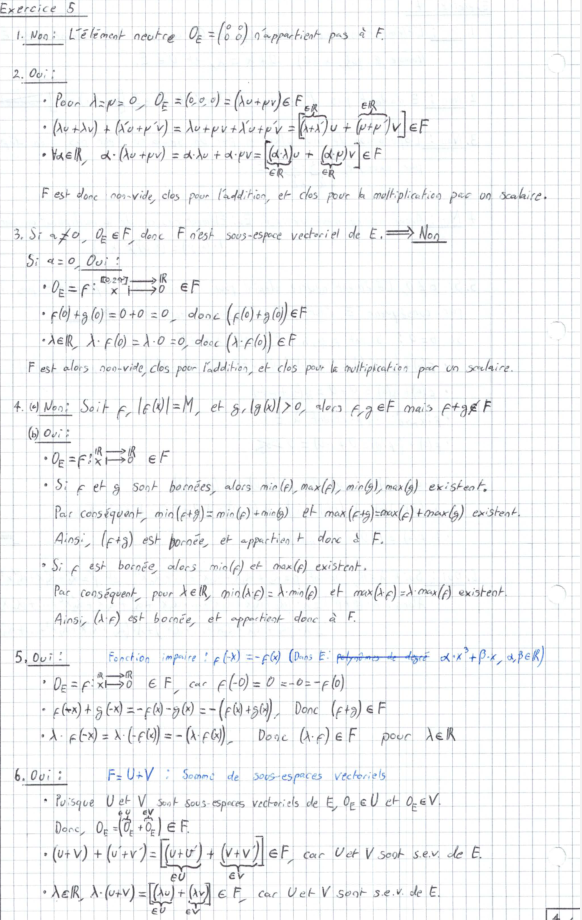
\includegraphics{ex05.png}
	
\end{document}
